% Comparing two inferences of one scene (oe_inferencex.compare, exp57 / exp58) with real rasters: Sen1Floods11 Bolivia
% tile 209, the S2 head against the S1 head on identical windows. Row 1: the two decisions, the disagreement windows on
% the scene, what they have in common (cue enrichment). Row 2: are two differences the same set (the phi matrix of the
% four Sen1Floods11 pairs), the two-date reading on GEOID-Flood, and the label bridge, boxed apart because it needs labels.
% Numbers come from rasters/cmp_numbers.tex, written by make_compare_rasters.py from the committed artifacts.
% Build: pdflatex compare_inferences.tex; export: osascript -l JavaScript pdf2png.js compare_inferences.pdf ../compare.png 3600
\documentclass[tikz,border=3mm]{standalone}
% Shared style for the diagrams: layered slanted rasters with shadows, geometric model parts, few words.
\usepackage{graphicx}
\pagecolor{white}   % an explicit page background: transparent pages export as black in some rasterisers
\usetikzlibrary{positioning,arrows.meta,shadows,shapes.geometric,calc,fit,backgrounds}
\definecolor{ink}{HTML}{1F2937}
\definecolor{muted}{HTML}{6B7280}
\definecolor{oeteal}{HTML}{0F766E}
\definecolor{oeamber}{HTML}{D97706}
\definecolor{oeviolet}{HTML}{6D28D9}
\definecolor{oeblue}{HTML}{2563EB}
\definecolor{oered}{HTML}{DC2626}
\newlength{\rw}\setlength{\rw}{2.3cm}   % raster width on the page (before the slant)
\tikzset{
  >=Stealth, font=\small,
  plane/.style={inner sep=0pt, outer sep=0pt, transform shape, yscale=0.55, yslant=0.35, draw=ink!60, line width=0.4pt,
                drop shadow={shadow xshift=0.7mm, shadow yshift=-0.7mm, opacity=0.25}},
  flat/.style={inner sep=0pt, outer sep=0pt, draw=ink!60, line width=0.4pt, drop shadow={shadow xshift=0.7mm, shadow yshift=-0.7mm, opacity=0.25}},
  lab/.style={font=\scriptsize, text=ink, inner sep=1pt, align=center},
  sub/.style={font=\scriptsize, text=muted, inner sep=1pt, align=center},
  part/.style={draw=ink, line width=0.6pt, drop shadow={shadow xshift=0.8mm, shadow yshift=-0.8mm, opacity=0.3}},
  card/.style={draw=ink!70, fill=white, rounded corners=2pt, line width=0.5pt, inner sep=4pt, drop shadow={shadow xshift=0.8mm, shadow yshift=-0.8mm, opacity=0.25}},
  flow/.style={->, line width=0.9pt, draw=ink},
  cell/.style={draw=oeamber, line width=0.9pt, fill=none},
  errcell/.style={draw=oered, line width=0.6pt, fill=none},
}
% \raster{name}{x}{y}{file}: one slanted raster plane centred at (x, y)
\newcommand{\raster}[4]{\node[plane] (#1) at (#2,#3) {\includegraphics[width=\rw]{rasters/#4}};}
% \flatraster{name}{x}{y}{file}{width}: an unslanted raster
\newcommand{\flatraster}[5]{\node[flat] (#1) at (#2,#3) {\includegraphics[width=#5]{rasters/#4}};}
% \cells{plane node}{grid size}{style}{list macro}: outline windows r/c of a G x G grid on a slanted plane
\newcommand{\cells}[4]{%
  \begin{scope}[shift={(#1.center)}, yscale=0.55, yslant=0.35]
    \pgfmathsetlengthmacro{\cw}{\rw/#2}
    \foreach \r/\c in #4 {
      \draw[#3] ({(\c-#2/2)*\cw}, {(#2/2-\r-1)*\cw}) rectangle ++(\cw, \cw);
    }
  \end{scope}}
% same on a flat raster of width #5
\newcommand{\flatcells}[5]{%
  \begin{scope}[shift={(#1.center)}]
    \pgfmathsetlengthmacro{\cw}{#5/#2}
    \foreach \r/\c in #4 {
      \draw[#3] ({(\c-#2/2)*\cw}, {(#2/2-\r-1)*\cw}) rectangle ++(\cw, \cw);
    }
  \end{scope}}
% three-plane stack: \stack{prefix}{x}{y}{back}{mid}{front}
\newcommand{\stack}[6]{\raster{#1back}{#2}{#3}{#4}\raster{#1mid}{#2+0.15}{#3+0.75}{#5}\raster{#1}{#2+0.3}{#3+1.5}{#6}}
% Encoder and decoder are trapezoids in opposite directions (rule from the user, 2026-09-08):
% \encoderShape{name}{x}{y}{width}{height}{fill}: wide at the left, narrow at the right (in -> compressed)
% \decoderShape{name}{x}{y}{width}{height}{fill}: narrow at the left, wide at the right (compressed -> out)
\newcommand{\encoderShape}[6]{%
  \draw[part, fill=#6] (#2,#3-#5/2) -- (#2,#3+#5/2) -- (#2+#4,#3+#5/4) -- (#2+#4,#3-#5/4) -- cycle;
  \coordinate (#1) at (#2+#4/2,#3); \coordinate (#1in) at (#2,#3); \coordinate (#1out) at (#2+#4,#3);}
\newcommand{\decoderShape}[6]{%
  \draw[part, fill=#6] (#2,#3-#5/4) -- (#2,#3+#5/4) -- (#2+#4,#3+#5/2) -- (#2+#4,#3-#5/2) -- cycle;
  \coordinate (#1) at (#2+#4/2,#3); \coordinate (#1in) at (#2,#3); \coordinate (#1out) at (#2+#4,#3);}

\usepackage{amssymb}
\def\cmpEvent{EMSR275-1}
\def\cmpDatePre{2017-07-07}
\def\cmpDatePost{2018-03-22}
\def\cmpChip{2293}
\def\cmpChipDisagree{152}
\def\cmpChipWindows{196}
\def\cmpChipRate{78}
\def\cmpChipFlooded{84}
\def\cmpChipErrA{0}
\def\cmpChipErrB{16}
\def\cmpPooledRate{3.4}
\def\cmpPooledWindows{870,728}
\def\cmpEvents{55}
\def\cmpEventRateMedian{1.4}
\def\cmpEnrBoundary{10.1}
\def\cmpEnrLowConf{3.0}
\def\cmpEnrUnstable{2.9}
\def\cmpEnrNdwi{6.6}
\def\cmpShareBoundaryDis{19}
\def\cmpShareBoundaryAgr{1.9}
\def\cmpFloodedAll{27}
\def\cmpErrAAll{33}
\def\cmpErrBAll{40}
\def\cmpErrorsPhi{0.58}
\def\cmpEventPhiMedian{0.30}
\def\cmpBothShare{41}
\def\cmpBothFlooded{52}
\def\cmpBothEventsW{16}
\def\cmpBothEventsL{9}
\def\cmpRuleFlooded{80}
\def\cmpRuleShare{6}
\def\cmpChipBothFlooded{100}
\def\cmpPhiNames{0/offsets, 1/backbones, 2/sensors, 3/fine-tune}
\def\cmpPhiCells{0/0/1.00, 0/1/0.29, 0/2/0.20, 0/3/0.28, 1/0/0.29, 1/1/1.00, 1/2/0.27, 1/3/0.28, 2/0/0.20, 2/1/0.27, 2/2/1.00, 2/3/0.31, 3/0/0.28, 3/1/0.28, 3/2/0.31, 3/3/1.00}

\def\cmpDisagree{4/8}

\def\cmpDisagreeBoundary{1/9, 2/1, 2/5, 2/8, 2/9, 3/2, 3/6, 3/9, 4/2, 4/12, 4/13, 5/2, 5/14, 6/1, 6/14, 8/2, 9/8, 10/1, 10/7, 10/9, 12/6, 13/5, 13/6, 14/5}

\def\cmpARight{2/1, 2/8, 3/2, 3/9, 4/2, 4/8, 5/2, 6/1, 8/2, 9/8, 10/1, 10/7, 12/6, 13/5, 13/6, 14/5}

\def\cmpBRight{1/9, 2/5, 2/9, 3/6, 4/12, 4/13, 5/14, 6/14, 10/9}

\tikzset{lab/.style={font=\small, text=ink, inner sep=1pt, align=center},
         sub/.style={font=\footnotesize, text=muted, inner sep=1pt, align=center},
         tag/.style={font=\footnotesize, text=ink, fill=white, fill opacity=0.85, text opacity=1, inner sep=1.5pt, rounded corners=1pt},
         dcell/.style={draw=oeamber, line width=0.9pt, fill=none},
         bcell/.style={draw=oered, line width=0.9pt, fill=none},
         acell/.style={draw=oeteal, line width=0.6pt, fill=oeteal, fill opacity=0.55},
         rcell/.style={draw=oeviolet, line width=0.6pt, fill=oeviolet, fill opacity=0.55},
         labelled/.style={card, draw=oeviolet!80, dashed}}
\begin{document}
\begin{tikzpicture}
  % ================= row 1: the scene, two inferences, the disagreement windows, what they have in common
  \flatraster{scene}{1.3}{5.8}{cmp_rgb.png}{2.4cm}
  \node[lab] at (1.3,7.75) {one scene};
  \node[sub] at (1.3,4.3) {Sentinel-2, Bolivia tile \cmpTile};
  \flatraster{ma}{4.35}{5.8}{cmp_a.png}{2.0cm}
  \flatraster{mb}{6.65}{5.8}{cmp_b.png}{2.0cm}
  \node[lab] at (5.5,7.75) {two inferences, same windows};
  \node[sub] at (4.35,4.55) {A: S2 head};
  \node[sub] at (6.65,4.55) {B: S1 head};
  \draw[flow] (2.55,5.8) -- (3.3,5.8);
  \flatraster{dis}{10.3}{5.8}{cmp_rgb.png}{3.2cm}
  \flatcells{dis}{16}{dcell}{\cmpDisagree}{3.2cm}
  \flatcells{dis}{16}{bcell}{\cmpDisagreeBoundary}{3.2cm}
  \draw[flow] (7.7,5.8) -- (8.65,5.8);
  \node[lab] at (10.3,7.75) {where A and B differ, no labels};
  \node[sub] at (10.3,4.0) {\cmpTileDisagree{} of \cmpTileWindows{} windows on this tile (\cmpTileRate\%),\\ \cmpPooledRate\% of \cmpPooledWindows{} over the testbed};
  \node[tag, anchor=south east] at ($(dis.south east)+(-0.08,0.08)$) {\textcolor{oered}{$\square$} on a boundary of A};
  % evidence card: the cues' share among disagreement windows over their share among agreement windows
  \node[card] (ev) at (17.2,5.8) {%
    \begin{tikzpicture}[font=\scriptsize, x=0.42cm]
      \foreach \name/\y/\e in {boundary/0/\cmpEnrBoundary, low conf./-0.7/\cmpEnrLowConf, unstable/-1.4/\cmpEnrUnstable, NDWI $\approx 0$/-2.1/\cmpEnrNdwi} {
        \node[sub, anchor=west] at (0,\y) {\name};
        \fill[oeteal!70] (2.6,\y-0.16) rectangle ({2.6+\e},\y+0.16);
        \node[lab, anchor=west] at ({2.6+\e+0.12},\y) {\e$\times$};
      }
      \draw[muted, line width=0.4pt] (2.6,0.4) -- (2.6,-2.45);
      \node[sub, anchor=west] at (0,0.7) {share among disagreement windows /};
      \node[sub, anchor=west] at (0,0.4) {share among agreement windows};
      \node[sub, anchor=west] at (0,-2.75) {boundary: \cmpShareBoundaryDis\% of the disagreement windows, \cmpShareBoundaryAgr\% of the rest};
    \end{tikzpicture}};
  \node[lab] at (17.2,7.75) {what they have in common};
  \draw[flow] (11.95,5.8) -- (ev.west);
  % ================= row 2: stability, the two-date reading, the label bridge
  \node[card] (stab) at (10.3,1.15) {%
    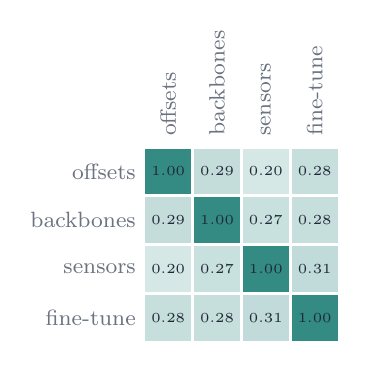
\begin{tikzpicture}[font=\scriptsize]
      \foreach \i/\j/\v in \cmpPhiCells {
        \pgfmathsetmacro{\lvl}{min(100, \v*85)}
        \fill[oeteal!\lvl] ({\j*0.62},{-\i*0.62}) rectangle ++(0.58,0.58);
        \node[font=\tiny, text=ink] at ({\j*0.62+0.29},{-\i*0.62+0.29}) {\v};
      }
      \foreach \i/\n in \cmpPhiNames {
        \node[sub, anchor=east] at (-0.08,{-\i*0.62+0.29}) {\n};
        \node[sub, anchor=west, rotate=90] at ({\i*0.62+0.29},0.7) {\n};
      }
    \end{tikzpicture}};
  \node[lab] at (10.3,3.15) {are two differences the same set?};
  \node[sub] at (10.3,-1.6) {phi between four pairs' disagreement sets:\\ different differences (median 0.28);\\ the same pair across head draws: \cmpDrawsPhi};
  \draw[flow] (10.3,3.95) -- (10.3,3.45);
  % the two-date reading: GEOID-Flood, the pre-event S2 head against the post-event S1 head, per event
  \node[card, text width=5.3cm, align=left, font=\footnotesize] (geo) at (4.4,1.15) {%
    \textbf{two dates of one scene} (GEOID-Flood, \cmpGeoEvents{} events): pre-event S2 head against post-event S1 head.\\[2pt]
    \cmpGeoRate\% of the windows differ, \cmpGeoBoundaryEnr$\times$ boundary-enriched. Both sides confident on \cmpGeoBothShare\% of them: those are flooded by the label \cmpGeoFloodedBoth\% of the time, against \cmpGeoFloodedAll\% of all differing windows.\\[2pt]
    \textcolor{muted}{a reading of the difference, not a proof of change (exp58)}};
  \node[lab] at (4.4,3.15) {the same measurement across time};
  % the label bridge: boxed apart, dashed, because it needs labels
  \node[labelled] (lb) at (17.2,1.15) {%
    \begin{tikzpicture}
      \flatraster{lt}{0}{0}{cmp_rgb.png}{2.5cm}
      \flatcells{lt}{16}{acell}{\cmpARight}{2.5cm}
      \flatcells{lt}{16}{rcell}{\cmpBRight}{2.5cm}
      \node[sub, anchor=west, align=left] at (1.45,0.6) {\textcolor{oeteal}{$\blacksquare$} A right: \cmpARightShare\%};
      \node[sub, anchor=west, align=left] at (1.45,0.15) {\textcolor{oeviolet}{$\blacksquare$} B right: \cmpBRightShare\%};
      \node[sub, anchor=west, align=left] at (1.45,-0.35) {error maps phi \cmpErrorsPhi};
      \node[sub, anchor=west, align=left] at (1.45,-0.8) {(testbed, hand labels)};
    \end{tikzpicture}};
  \node[lab, text=oeviolet] at (17.2,3.15) {which side is right: with labels only};
  \draw[flow, draw=oeviolet, dashed] (17.2,3.9) -- (17.2,3.45);
\end{tikzpicture}
\end{document}
